\subsection{Theory}
\label{section:XPS}\index{XPS} XPS is a tool to achieve information of the samples chemical structure.
\footnote{Most of the information given here is taken from \cite{Riviere_90} in \cite{briggs_auger_1990}.}
When X-rays with sufficient energy hit metals, electrons are emitted. This effect is called photoelectric effect and was first discovered by Heinrich Hertz in 1887 through the fact that electrodes illuminated with ultraviolet light create electric sparks more easily\cite{hertz_ueber_1887}. 18 years later Albert Einstein received the Nobel Price for his discovery of the law of the photoelectric effect\cite{_nobel_2015} and a scientific explanation which Hertz was missing.

The standard X-ray source is supplied with aluminum and magnesium anodes. \footnote{Other materials are available that produce various X-ray energies and line widths \index{XPS!Anode materials} \cite{_x-ray_2015}.}
\begin{table}\caption{Energy and line widths of some anode materials. Taken from \cite{_x-ray_2015}}
	\centering
	\begin{tabular}{cccc}
		Anode 	& 	Radiation 	& Photon Energy (eV) 	& Line Width (eV) \\ \hline
		Mg	&	K$\alpha$ 	&	1253.6	&	0.7\\
		Al	&	K$\alpha$ 	&	1486.6 	&	0.85\\
	\end{tabular}
\end{table}

\index{XPS!Physical model}As the X-rays hit and penetrate the sample surface they excite electrons and initiate different processes. The meajor two are discussed in the following.

For the \textbf{core-level excitation} the X-ray removes a single electron next to the core which is then detected. Energy conservation due to elastic scattering of the electron out of the bulk results in the relation 
\begin{align}
%E_{kin} &= h\nu_{\textnormal{X-ray}}-E_{B}-\Phi_{\textnormal{analyzer}} \\
E_B 	&=h\nu_{\textnormal{X-ray}}-E_{kin}-\Phi_{\textnormal{analyzer}}
\end{align}
 $h\nu_{\textnormal{X-ray}}$ is the energy of the incident X-ray beam, $E_B$ the binding energy of the excited electron and $\Phi_{analyzer}$ the work function of the analyzer. 
 
% In the \textbf{Auger process} \index{XPS!Auger process} on the other hand the created core level (lets say at level K) vacancy is filled with a energetically higher lying electron (at for example level $L_1$). The excess energy can either be radiated away (X-ray fluorescence) or given to an electron in the same or in a more shallow level (lets say $L_{2,3}$). This electron then can leave the sample as Auger electron. Figure \ref{fig:XPS-auger} shows the mentioned process. 
 
% Due to the fact that this process has two stages these electrons are referred to as secondary electrons. The notation for this process is $KL_1L_{2,3}$. The electron taking part in the Auger process can also originate from within the valence band ($KL_{2,3}V$) or even both electrons may stem from the valence band ($KVV$). For every element there is a unique series of Auger excitations. This holds even if one or even both electrons come from a valence band, as the dominating term will always be the binding energy $E_K$. As the Auger energy $$E_{KL_1L_{2,3}}=E_K-E_{L_1}-E_{L_{2,3}}$$ is not a function of the excitation energy it will not shift when changing the X-ray energy. Even very heavy elements (as the number of atomic levels the possible Auger transitions increases) do not exhibit a very large number of Auger emission lines due to the fact that the transition probability favors only a few of this many. \cite{Briggs_90}

\begin{figure}\centering
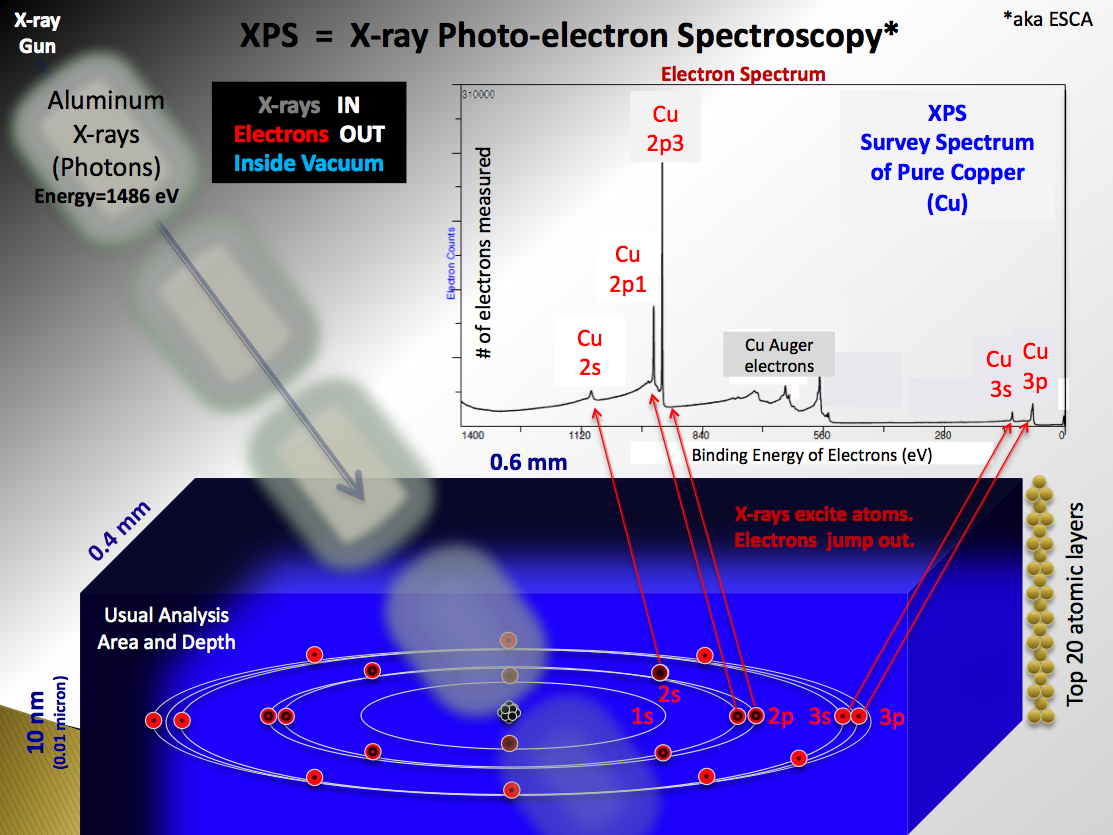
\includegraphics[width=0.45\textwidth]{./images/XPS_PHYSICS}
		\label{fig:XPS-excitation}
	%	\subfigure[Single step core electron emission after excitation with X-rays leads to detection of core electron binding energy. \cite{_whatisxps-04.jpg_2015}]{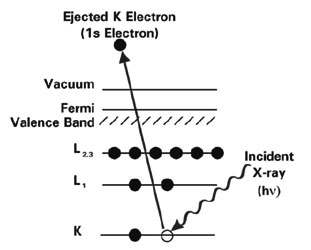
\includegraphics[height=0.3\textwidth]{./images/whatisxps-04.jpg}
	%		\label{fig:XPS-analyzer}}
	%	
%	\subfigure[Two step Auger process. In contrast to a direct emission of a core electron, the Auger emission involves more  electrons from less bound states. Here an ($L_{1}$) electron fills the hole in the $K$ shell created by the initial X-ray. The resulting hole in the $L_1$ shell is then filled with an $L_{2,3}$ electron resulting in a typical Auger emission feature. Adopted from \cite{Briggs_90}.]{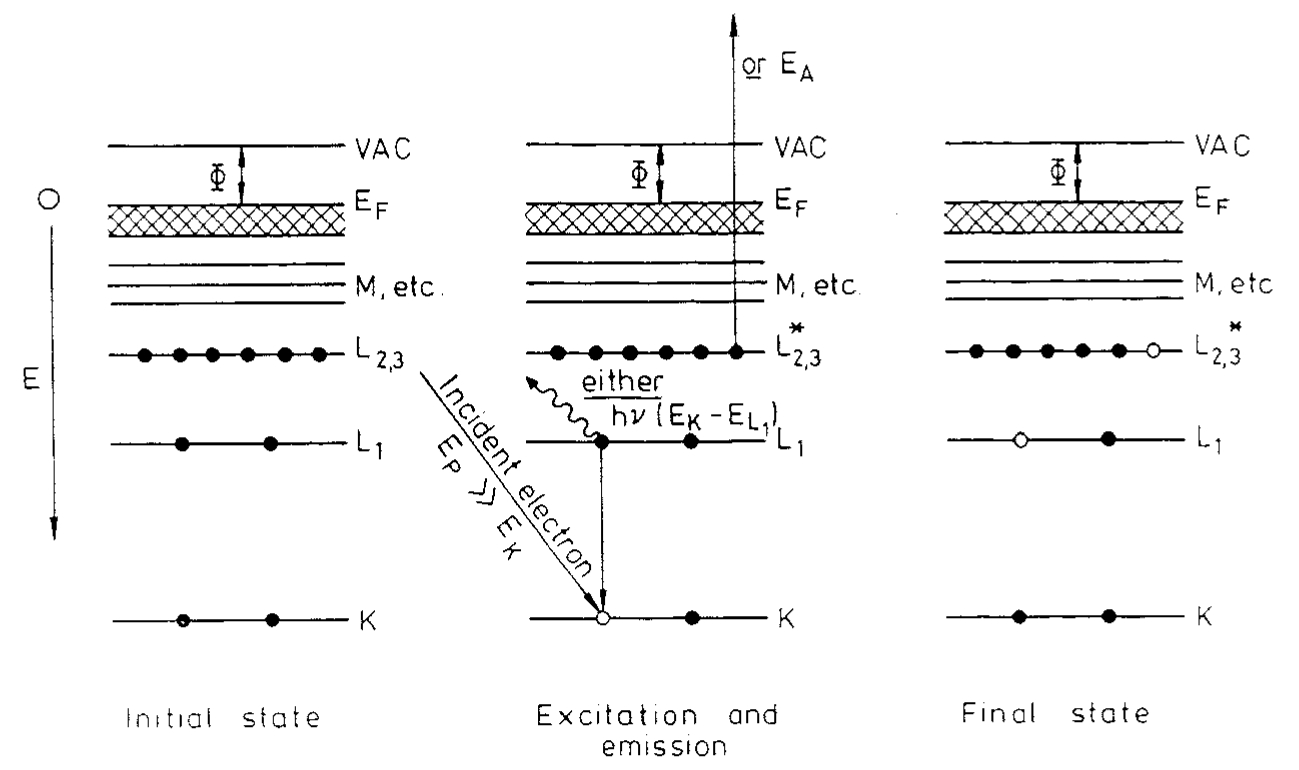
\includegraphics[width=0.45\textwidth]{./images/auger.jpg}
%		\label{fig:XPS-auger}}
	
	\caption{Representation of XPS process. A scheme of an X-ray gun illuminating a sample area of about \SI{0.4}{\milli \meter} x \SI{0.6}{\milli \meter} is shown. X-rays are used to excite core level electrons. Excited electrons within the first 20 layer escape the sample. After leaving the sample these show element specific signatures in their kinetic energies. A detailed analysis of the peak shape and shift allows for identification of the chemical environment.}
	\label{fig:auger-core}
\end{figure}

\cite{zemlyanov_versatile_2018}
The \index{XPS!chemical surrounding} chemical surrounding of atoms changes their binding energy, making XPS an ideal tool to detect changes in chemical surrounding. Although the analysis is averaged over the area of the incident X-rays its results are very precise. This makes it possible to distinguish differently bound atoms within single atomic species and therefore gives rise to otherwise not directly observable processes like growth, intercalation, etching and binding of for example graphene islands on Ir(111)\cite{busse_graphene_2011-1,granas_oxygen_2012}. XPS is used to identify oxidation processes of copper surfaces as the interaction of oxygen with the copper surface changes the Cu core level. \cite{deroubaix_x-ray_1992}.

%For the ease of analysis, many spectra are recorded with monochromatic radiation. This selects a certain energy for the following illumination of the sample. This technique relies on the dispersion of X-rays within a crystal. It is described by the Bragg relation $n\lambda = 2d\sin(\theta)$ where n is the diffraction order, $\lambda$ the wavelength of monochromatic radiation, d the distance between two crystal layers and $\theta$ is the so called Bragg angle. The first order peak for Al $K\alpha$ radiation ($\lambda=\SI{0,83}{\nm}$, $E=\SI{1486,6}{\eV}$) is at $\theta=\SI{78.5}{\degree}$ (using the $10\bar10$ planes of a quartz crystal with $d=\SI{0,425}{\nm}$). Therefore the angle between incident and reflected beam is about \SI{23}{\degree}.\cite{Riviere_90}

The spectra used in this work are recorded without monochromatic radiation as not stated otherwise. This is because the electron intensity is attenuated when using a monochromatic source.

The \index{XPS!binding energies} binding energies of some observed peaks are given in \autoref{tab:XPS-intensities}.
\begin{table}\centering
 \caption{Element specific transitions and binding energies for some chosen elements as reported in \cite{wanger_handbook_1979}}
 \begin{tabular}{lll}
  Eelement & excited state & $E_B$ [eV]\\ \hline 
  O & 1s & 531\\
  N & 1s & 398.1\\
  C & 1s & 285\\
  B & 1s & 189.4 \\
%  Cu & 2p $\frac{1}{2} (\frac{3}{2})$ & 953 (933) \\
%  Cu & LMM & 560-580 \\
  Cu & 3s & 123\\
  Cu & 3p $\frac{1}{2} (\frac{3}{2})$ & 77 (75)\\
 \end{tabular}
\label{tab:XPS-intensities}
\end{table}

\paragraph{Singlet/Multiplets}\index{XPS!Peak shapes}
The shape of the peaks typically resembles the line shape of the used X-rays (Gauss width $\approx 1eV$). In case of s-states $(l=0)$ (B1s, N1s, C1s) the peaks are singlets. With increasing $j=l+s$, the spin-orbit (j-j) coupling introduces a 'parallel' and 'anti-parallel' nature of the spin, resulting in two different $j=1/2(3/2)$ and therefore two different energies. The split in energy is expected to increase as Z increases (for constant n,l) or as l decreases (n constant). This makes the splitting of 3p orbitals larger than that of the 3d's. The ratio of the two peaks is given by their degeneracy $(2j+1)$.\cite[113]{Riviere_90}
\begin{table}
\caption{Spin-orbit splitting parameters. Ratios are reproduced from \cite{Riviere_90}}
\centering
 \begin{tabular}{ccc}
 Subshell & j values & Area ratio \\ \hline
 s & $\frac{1}{2}$ & --- \\
 p & $\frac{1}{2}$,$\frac{3}{2}$ & 1:2 \\
% d & $\frac{3}{2}$,$\frac{5}{2}$ & 2:3 \\
% f & $\frac{5}{2}$,$\frac{7}{2}$ & 3:4 \\
 \end{tabular}
\end{table}

\index{XPS!quantitative analysis}
%The more atoms of a specific kind are present, the larger the signal gets. Therefore the signal intensity resembles the amount of atoms on the topmost surface layers($\approx \SI{10}{\nm}$).
%
%As each irradiated atomic species has a different cross section for adsorption of X-rays with a certain energy they emit auger and core level spectra with a different intensity. Comparing the cross section of e.g. N with B's, one can see that it it roughly \SIrange{3}{4}{times} as large (B: \SI{6,87e3}{\barn\per atom}, N: \SI{25,82e3}{\barn\per atom} for $\textnormal{Al} K_{\alpha}$)\cite{henke_x-ray_1993}. Meaning that the signal from the N is much stronger than that of the B, although their number of atoms is equal.

\subsection{Experimental details}
	\paragraph{How X-Rays are created}
With the use of aluminum X-ray sources, electrons are accelerated with typically \SI{15}{\keV} onto the target. Most of the created radiation goes into the principal characteristic line ($K\alpha_{1,2}$). Higher ones ($K\alpha_{3,4}$, $K\beta$) are also observed but with much lower intensities. In addition there is a continuous background called Bremsstrahlung extending up to the energy of the incident electron energy. This background is of no use for the XPS measurement and has to be subtracted in a more or less artificial way.
\paragraph{XRays penetrate the crystal bulk and excite electrons in deep layers}
The more atoms of a specific kind are present, the larger the signal gets. Therefore the signal intensity resembles the amount of atoms on the topmost surface layers($\approx \SI{10}{\nm}$).

As each irradiated atomic species has a different cross section for adsorption of X-rays with a certain energy they emit auger and core level spectra with a different intensity. Comparing the cross section of e.g. N with B's, one can see that it it roughly \SIrange{3}{4}{times} as large (B: \SI{6,87e3}{\barn\per atom}, N: \SI{25,82e3}{\barn\per atom} for $\textnormal{Al} K_{\alpha}$)\cite{henke_x-ray_1993}. Meaning that the signal from the N is much stronger than that of the B, although their number of atoms is equal.
\paragraph{How electrons are analyzed}
\textcolor{red}{\textbf{Describe analyzer}}

\subsection{Methods}
	\paragraph{Coverage analysis}
	
	Referring to \cite{ertl_low_1986} the fraction $\theta_A$ of an adsorbate A on a surface B can be calculated via
	\begin{equation}\label{eq:adlayer-coverage}
	\theta_A=\frac{I_AI_B^0\cdot \exp(\frac{a_A}{\lambda_A}\cos(\Theta))}{I_AI_B^0( \exp(\frac{a_A}{\lambda_A}\cos(\Theta))-1)+I_BI_A^0\cdot \exp(\frac{a_A}{\lambda_A}\cos(\Theta))}
	\end{equation}
	where the parameters are given in table \ref{tab:adlayer-coverage-parameters}.
	
	\begin{table}[h!]\centering
		\caption{Description of parameters used in equation
			\ref{eq:adlayer-coverage}}
		\label{tab:adlayer-coverage-parameters}
		\begin{tabular}{cc}
			Parameter & Annotation \\ \hline
			$I_A$	& integrated intensity of the adsorbate peak \\
			$I_A^0$ & cross section of element A \\
			$\lambda_A$ & mean free path of electrons in material A \\
			$a_A$ & thickness of adlayer \\
		\end{tabular}
	\end{table}
	
	The mean free path of electrons with energy E in a solid is given by $\lambda_M=\SI{0,41}{}\cdot a_M^{\SI{0,41}{}}\cdot E_M^{\SI{0,5}{}} $ where $a_M$ is the atomic size of M. 
	\textcolor{red}{\textbf{Give atomic size and resulting value}}
	
\subsection{Limitations}
\paragraph{Beam damage}
Since the X-Rays bear a considerable energy other effects than the excitation of core electrons is possible. Especially for long integration times of the analyzer (for elements with little cross section or very little surface coverage) the amount of deposited energy results in unwanted side reaction on the surface. It is possible to trigger a change in the chemical surrounding of the investigated element, causing chemical shifts that are not present in the pristine sample and change the XPS spectrum over time.

\paragraph{Space averaging technique}
XPS is a space averaging technique. First the X-Ray beam has an inherent width, the analysis area can't be chosen arbitrarily small. Second, X-Rays do excite electrons not only directly within the illuminated area, but penetrate the bulk and cause a cascade of transitions in the sample. The resulting information is always a mix between surface adsorbates and bulk elements.